\documentclass{article}
\usepackage{graphicx} % Required for inserting images
\usepackage{indentfirst}
\usepackage{hyperref}

\title{Limbaje Formale si Translatoare
\\
Proiect}

\author{Eusebiu-Ioan Florean
\\
Răzvan-Vasile Bumbu}

\date{May 2023}

\begin{document}

\maketitle

\newpage

\tableofcontents
\newpage
\large 

\section{Introducere}
In cadrul acestui proiect am realizat un mini-interpretor pentru un limbaj de programare propriu, care este capabil de asemenea sa execute si sa afiseze rezultatul codului introdus ca si input. \\

Interpretorul este în tehnică software (de programare), un program special prin care se citește, se analizează și se execută (interpretează pe loc) comenzile și instrucțiunile dintr-un program sursă - și anume pas cu pas, una după alta, fără o compilare anterioară. Eventualele erori de programare din programul-sursă devin evidente abia în momentul când interpretorul încearcă să-l execute și evident se blochează. \\

Interpretarea unui program sursă durează mai mult decât executarea programului (același) compilat. Aceasta se explică prin aceea că instrucțiunile unui program compilat sunt direct executate, în timp ce interpretorul citește și analizează mai întâi instrucțiunile, după care le poate executa.

\begin{center}
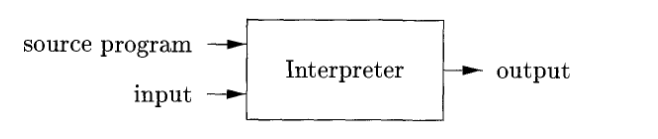
\includegraphics[]{interpretor.png}\\
\textit{Cun functioneaza un interpretor}
\end{center}


\section{Descrierea proiectului}

Limbajul propriu de programare are la baza 3 tipuri de variabile regasite in majoritatea limbajelor de programare imperative:
\begin{itemize}
    \item Numere intregi - \textbf{int}
    \item Numere reale - \textbf{float}
    \item Siruri de caractere - \textbf{string}\\
\end{itemize}


De asemenea, pe langa variabile, limbajul contine si o serie de instructiuni:
\begin{itemize}
    \item Instructiuni de selectie
    \begin{itemize}
        \item \textbf{if}
        \item \textbf{switch}
    \end{itemize}
    \item Instructiuni de ciclare
    \begin{itemize}
        \item \textbf{while}
        \item \textbf{do while (repeat until)}
        \item  \textbf{for}
    \end{itemize}
    \item Instructiuni de operatii aritmetice pe numere intregi si numere reale
    \begin{itemize}
        \item \textbf{+}
        \item \textbf{-}
        \item \textbf{*}
        \item \textbf{/}
        \item \textbf{=}
    \end{itemize}
    \item Instructiuni de operatii logice pe numere intregi si numere reale
    \begin{itemize}
        \item \textbf{$<$}
        \item \textbf{$>$}
        \item \textbf{$<=$}
        \item \textbf{$>=$}
        \item \textbf{$==$}
        \item \textbf{$!=$}
    \end{itemize}
    \item Instructiune de afisare output
    \begin{itemize}
        \item \textbf{print}
    \end{itemize}
\end{itemize}


In plus, am decis sa implementam in cadrul proiectului doua functionalitati diferite fata de limbajele de programare clasice. \\

O prima functionalitate este aceea a introducerii unei instructiuni care permite utilizatorului sa joace jocul Tic Tac Toe (X si O).\\

Cea de-a doua functionalitate adaugata, este una gandita pentru utilizarea interpretorului, si anume interfata web in care utilizatorul poate introduce codul sursa, dupa care, prin apasarea butonului pentru rulare, acesta va primi output-ul programului.\\

\textbf{OBSERVATII}
\begin{itemize}
    \item Variabilele pot fi declarate doar utilizand literele mici ale alfabetului englez \textbf{(a..z)}
    \item Declararea si instantierea variabilelor se va face exclusiv de forma:
    \textbf{\\tip nume; \\nume = valoare;}
    \item Instantierea numerelor reale se va face folosind simbolul \textbf{punct(.)} intre partea intreaga si partea fractionara.
    \item Instantierea sirurilor de caractere se va face folosind simbolurile \textbf{" "}.
    \item Sirurile de caractere nu trebuie sa contina o singura litera sau cuvinte rezervate pentru nume de variabile sau instructiuni si de asemenea nu pot sa contina spatii.
    \item Instructiunea \textbf{print} poate afisa doar valoarea unei singure variabile, fara alte mesaje.
    \item Instructiunea \textbf{if} trebuie sa contina cel mult o ramura \textbf{else}.
    \item Instructiunea \textbf{switch} trebuie sa contina doua ramuri \textbf{case} si o ramura \textbf{default}.
    \item Finalul codului se va marca prin simbolul \textbf{punct(.)}.
    \item Exemple pentru folosirea corecta a instructiunilor poate fi vazuta in sectiunea \textbf{4. Exemple de rulare}.
\end{itemize}

\begin{center}
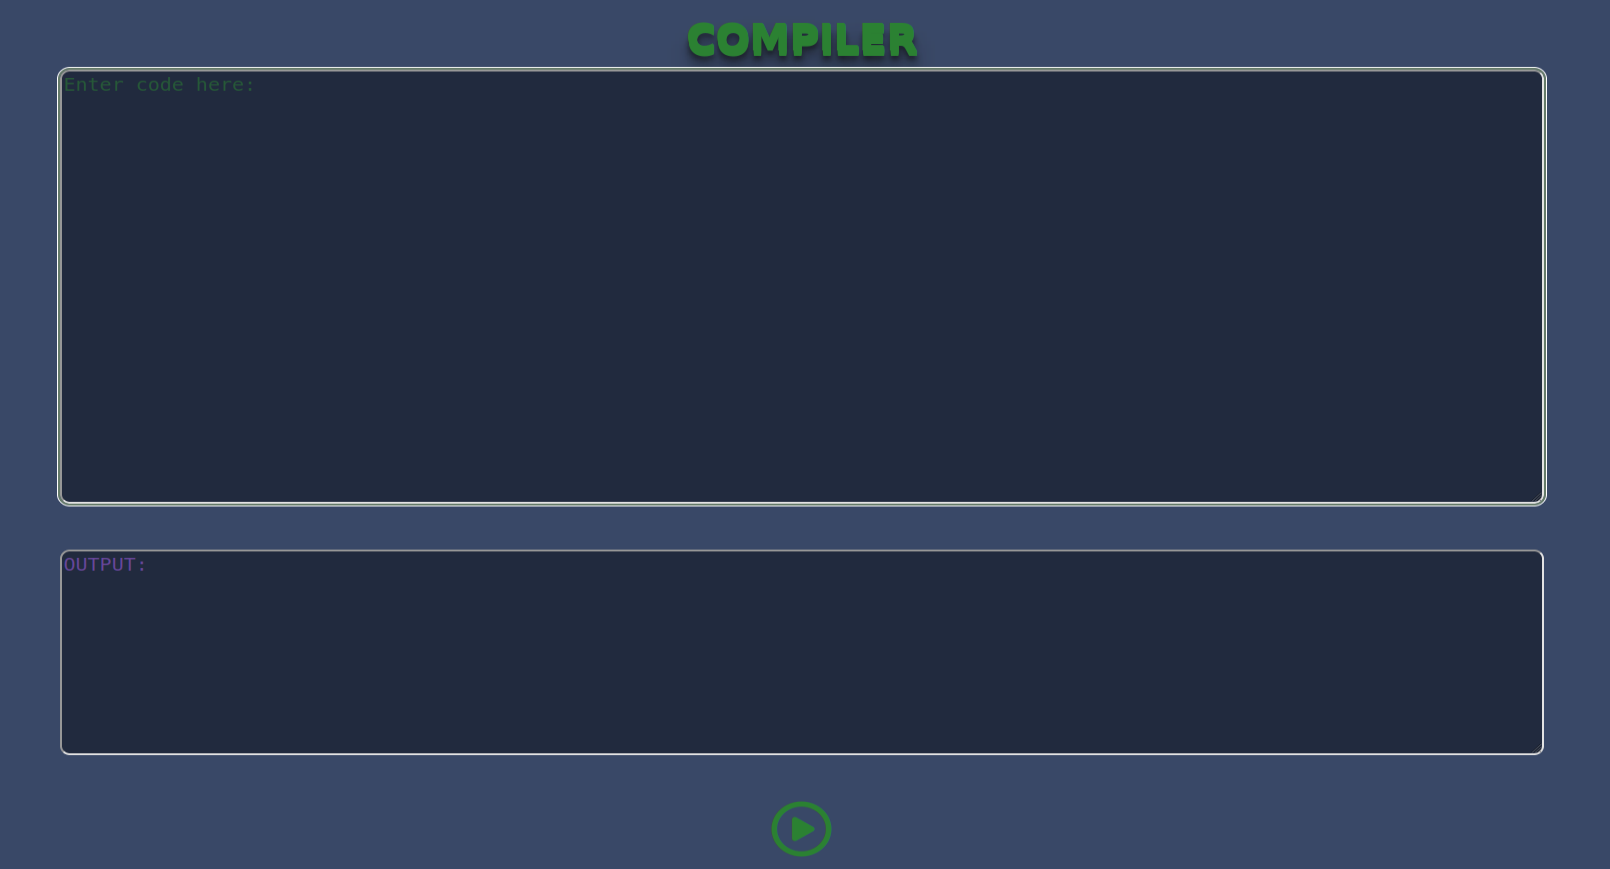
\includegraphics[scale = 0.4]{interfata grafica.png}\\
\textit{Interfata grafica a aplicatiei}
\end{center}


\section{Decizii de implementare}
Acest proiect a fost dezvoltat cu ajutorul mai multor limbaje de programare:
\begin{itemize}
\item \textbf{lex} 
\item \textbf{yacc}
\item \textbf{C}
\item \textbf{nodemon}
\item \textbf{HTML/CSS/JAVA SCRIPT} 
\end{itemize}

Prin lex are loc parsarea textului(codul sursa) spre yacc, generand tokeni prin expresiile regulate definite in fisierul "interpreter.l". Un exemplu de parsare, reprezentat prin imaginea de mai jos, este recunoasterea comenzilor de tipul "put on x y". In momentul in care va fi introdusa de catre utilizator o comanda analog acesteia, parserul o va valida, fiind vorba despre o comanda din jocul "tic tac toe", va seta in yylval.x pozitia liniei, in yylval.y pozititia coloanei dupa care va returna tokenul PUT care va fi interpretat ulterior de catre yacc. \\

\begin{center}
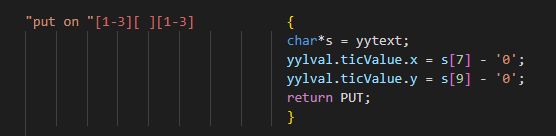
\includegraphics[scale = 0.4]{lex_example.png}\\
\textit{\textbf{parser.l} code-example}
\end{center}

In cadrul fisierului \textbf{interpreter.y} sunt definite functiile in limbajul C care vor fi apelate in momentul validarii tokenilor. Semnatura tuturor acestor functii, impreuna cu declaratiile de noi tipuri sunt definite in fisierul "types.h" care este importat pe urma in yacc. \\

Acest fisier contine marea majoritate a logicii, care consta in construirea arborelui de parsare, adaugandu-se cate un nou nod cu fiecare nou token parsat. Cand scanarea fisierului s-a terminat, adica exista un arbore complet, va fi apelata functia execute() care parcurge intregul arbore evaluand valoarea fiecarui nod. \\

Pentru printarea valorii unei variabile prin comanda \textbf{"print"} se acceseaza memoria in cadrul careia se pastreaza pentru fiecare variabila de la \textbf{'a}' la \textbf{'z'} tipul si valoarea. Se verifica \textbf{tipul} variabilei, dupa care are loc afisarea \textbf{valorii} acesteia prin utilizarea variabile aux de tipul data care reprezinta valoarea functiei apelate recursiv.

\begin{center}
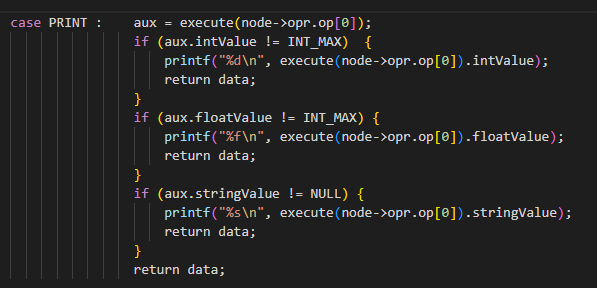
\includegraphics[scale = 0.4]{print_example.png}\\
\textit{\textbf{print} code-example}
\end{center}

Pentru recunoasterea structurilor de tip \textbf{if} are loc crearea unui nod in 2 cazuri:\\
\begin{itemize}
\item \textbf{if-then:} nod cu 2 copii: expresia si propozitia(then)
\item \textbf{if-then-else:} nod cu 3 copii: expresia si cele 2 propozitii (then si else)
\end{itemize}
O data creat acest nod, va fi recunoscut in functia execute unde se va distinge daca este un if cu sau fara ramura else in functie de numarul de copii ai nodului radacina, apelandu-se pentru fiecare caz codul C corespunzator.

\begin{center}
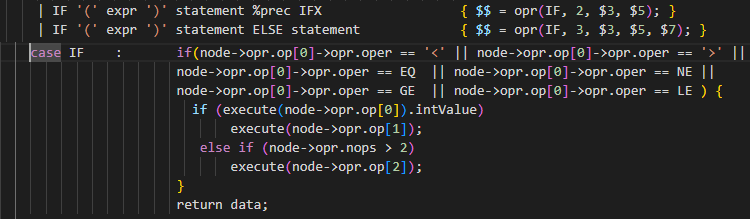
\includegraphics[scale = 0.4]{if_code_example.png}\\
\textit{\textbf{if-then-else} code-example}
\end{center}

Scheletul interfetei grafice a fost realizat in \textbf{HTML}, stilizat cu ajutorul \textbf{CSS}, iar pentru dinamicitatea elementelor grafice s-a folosit \textbf{Bootstrap}. \\

Partea de client a aplicatiei care se ocupa cu functionalitatii paginii web este dezvoltata in \textbf{Java Script}, care utilizeaza \textbf{web-sockets} pentru comunicarea cu server-ul \textbf{nodemon}. In momentul in care utilizatorul actioneaza butonul de rulare al programului, este preluat textul introdus de acesta in casuta de input si este transmis spre server\textbf{(I)}. Acesta citeste mesajul reprezentand programul scris de utilizator, il executa cu ajutorul fisierul yacc si lex, dupa care trimite ca raspuns clientului output-ul \textbf{(II)}, fiind preluat de catre client care va actualiza interfata grafica \textbf{(III)}.

\begin{center}
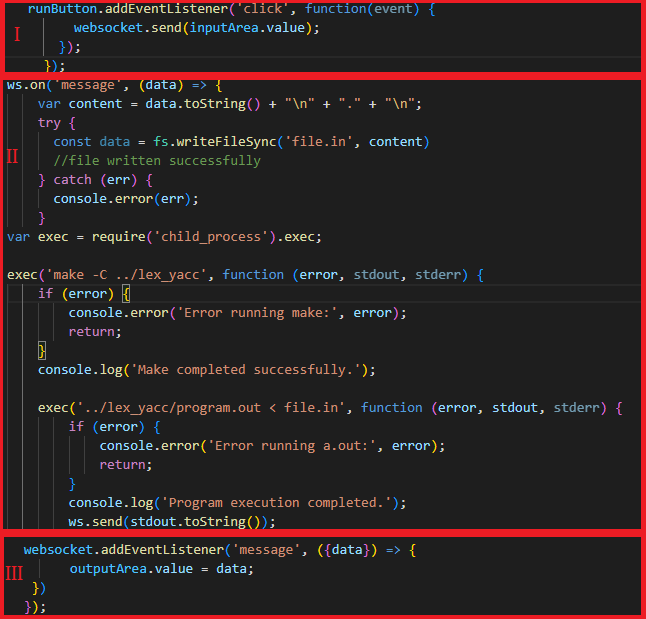
\includegraphics[scale = 0.4]{client_server_code_example.png}\\
\textit{\textbf{client server} code-example}
\end{center}

\section{Exemple de rulare}

\begin{center}
\inprimiti cludegraphics[scale = 0.4]{asignare.png}\\
\textit{Asignarea variabilelor}
\end{center}

\begin{center}
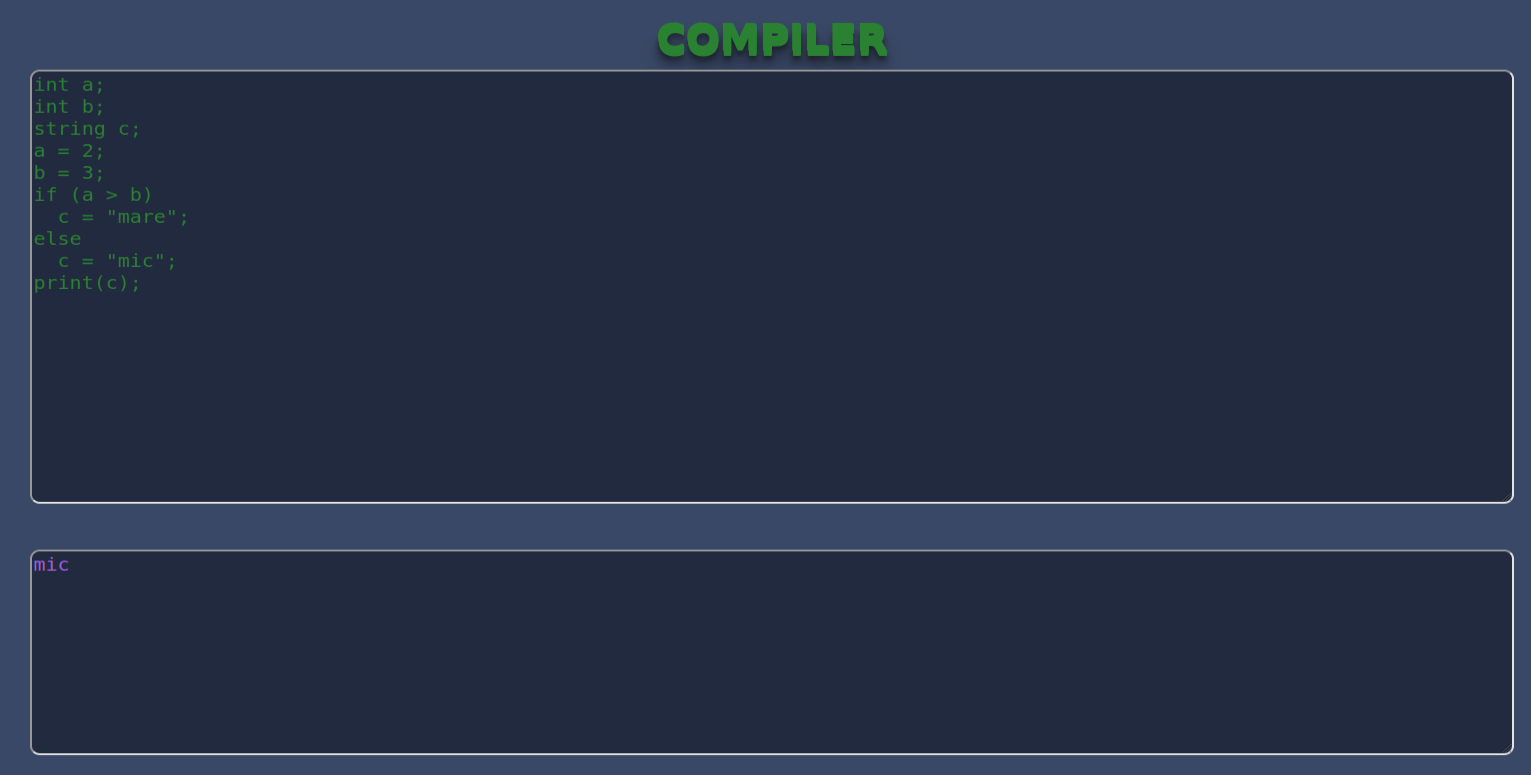
\includegraphics[scale = 0.4]{if.png}\\
\textit{Instructiunea \textbf{if}}
\end{center}

\begin{center}
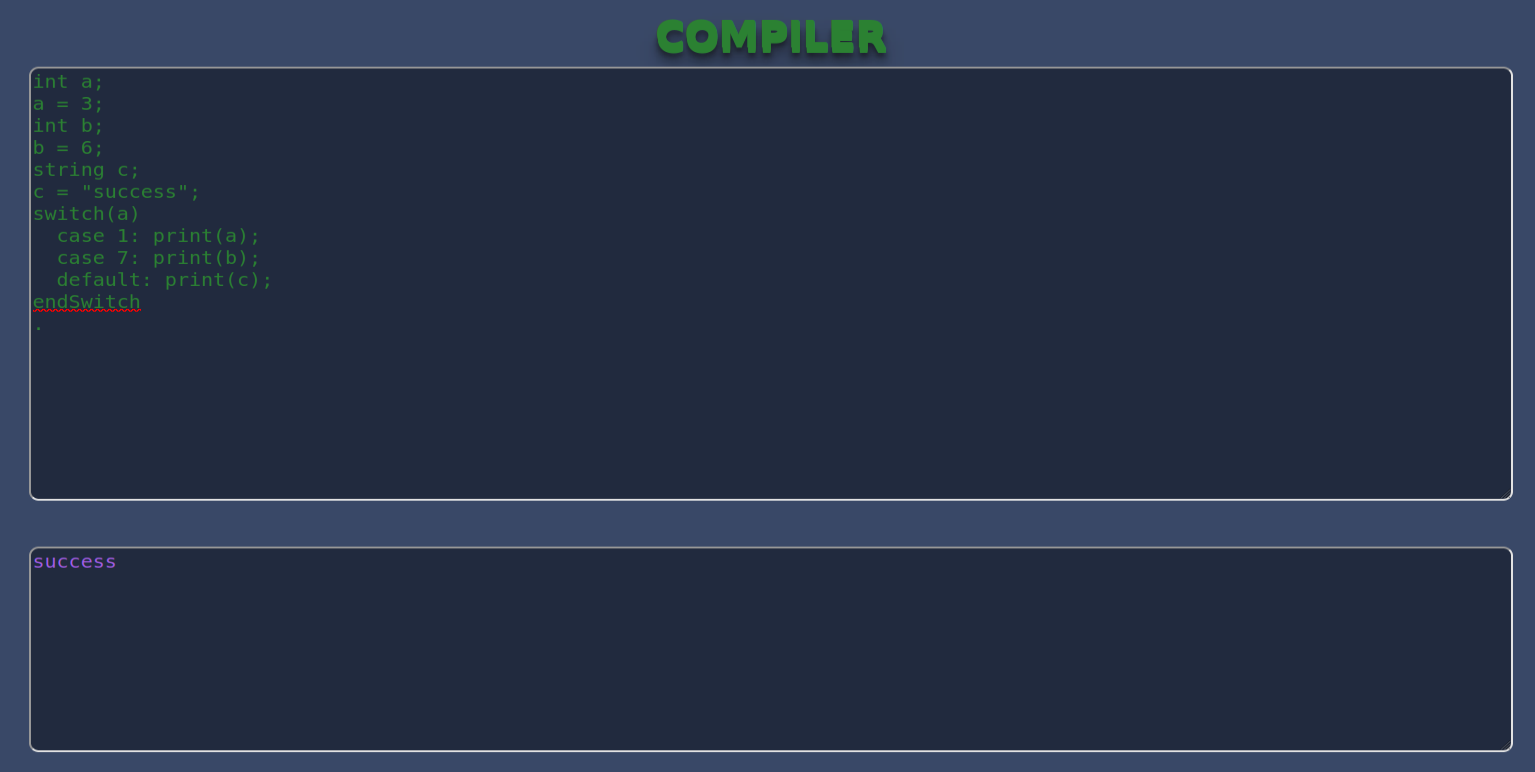
\includegraphics[scale = 0.4]{switch.png}\\
\textit{Instructiunea \textbf{switch}}
\end{center}

\begin{center}
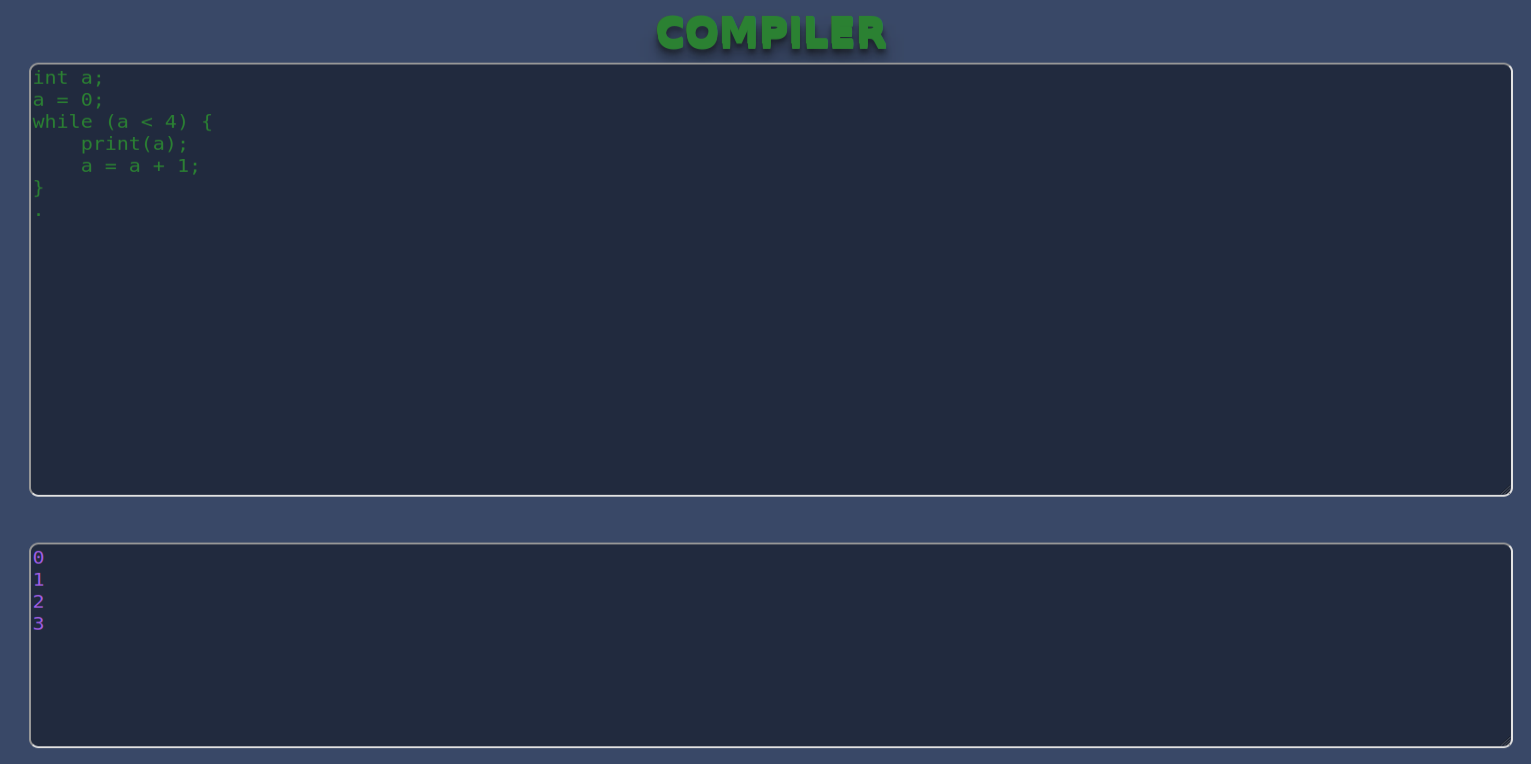
\includegraphics[scale = 0.4]{while.png}\\
\textit{Instructiunea \textbf{while}}
\end{center}

\begin{center}
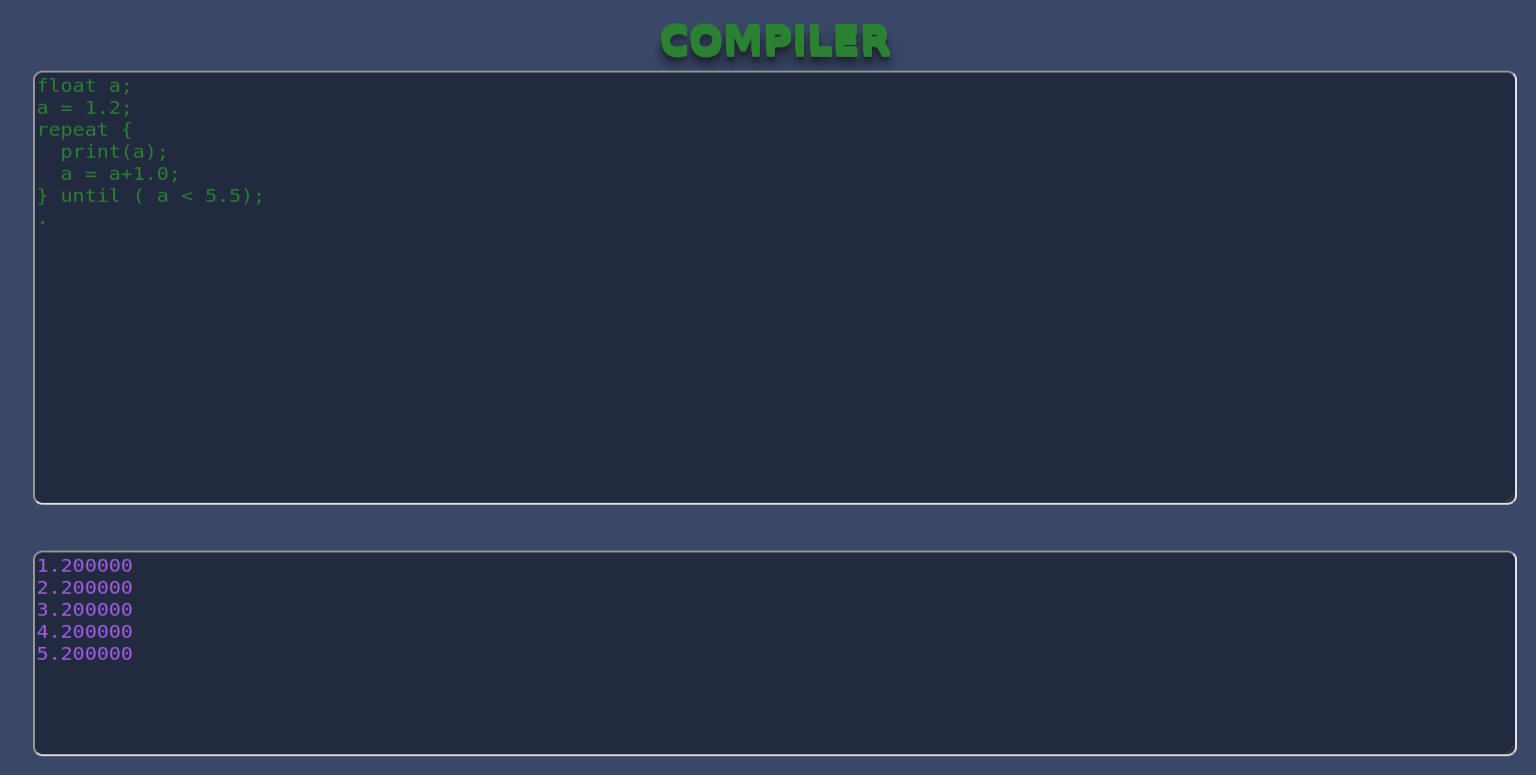
\includegraphics[scale = 0.4]{repeatUntil.png}\\
\textit{Instructiunea \textbf{repeat until}}
\end{center}

\begin{center}
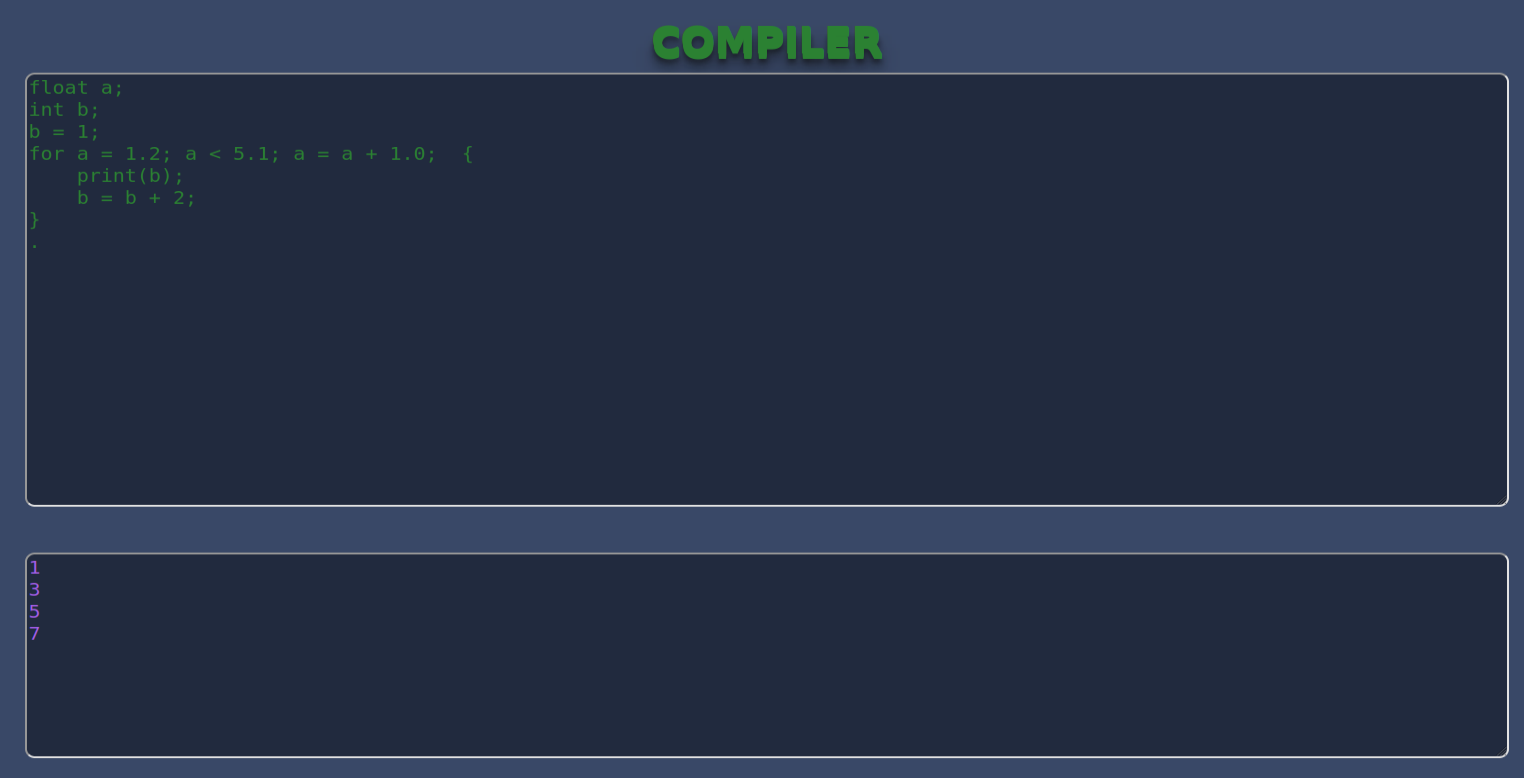
\includegraphics[scale = 0.4]{for.png}\\
\textit{Instructiunea \textbf{for}}
\end{center}

\begin{center}
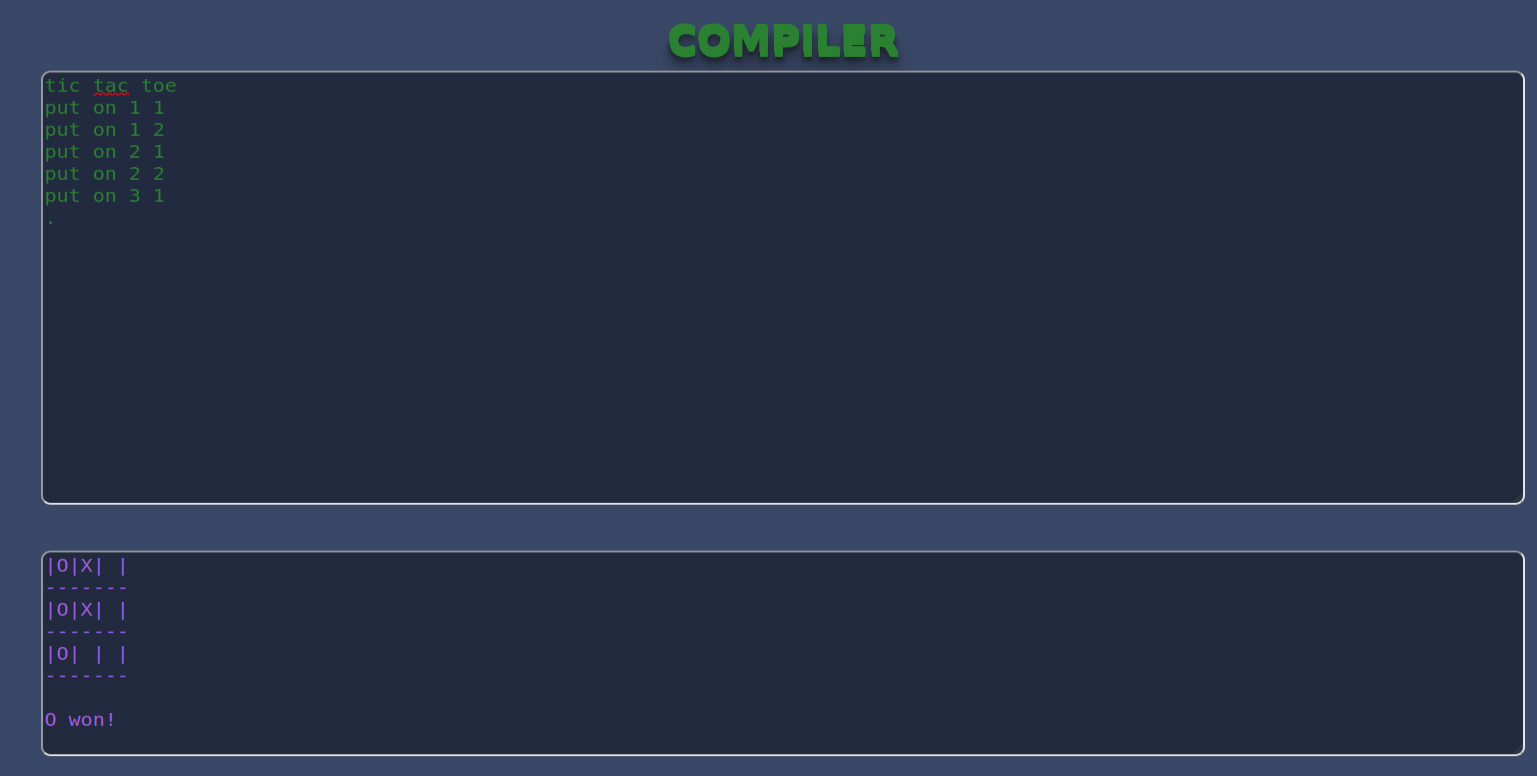
\includegraphics[scale = 0.4]{ticTacToe.png}\\
\textit{Instructiunea \textbf{Tic Tac Toe}}
\end{center}

\begin{center}
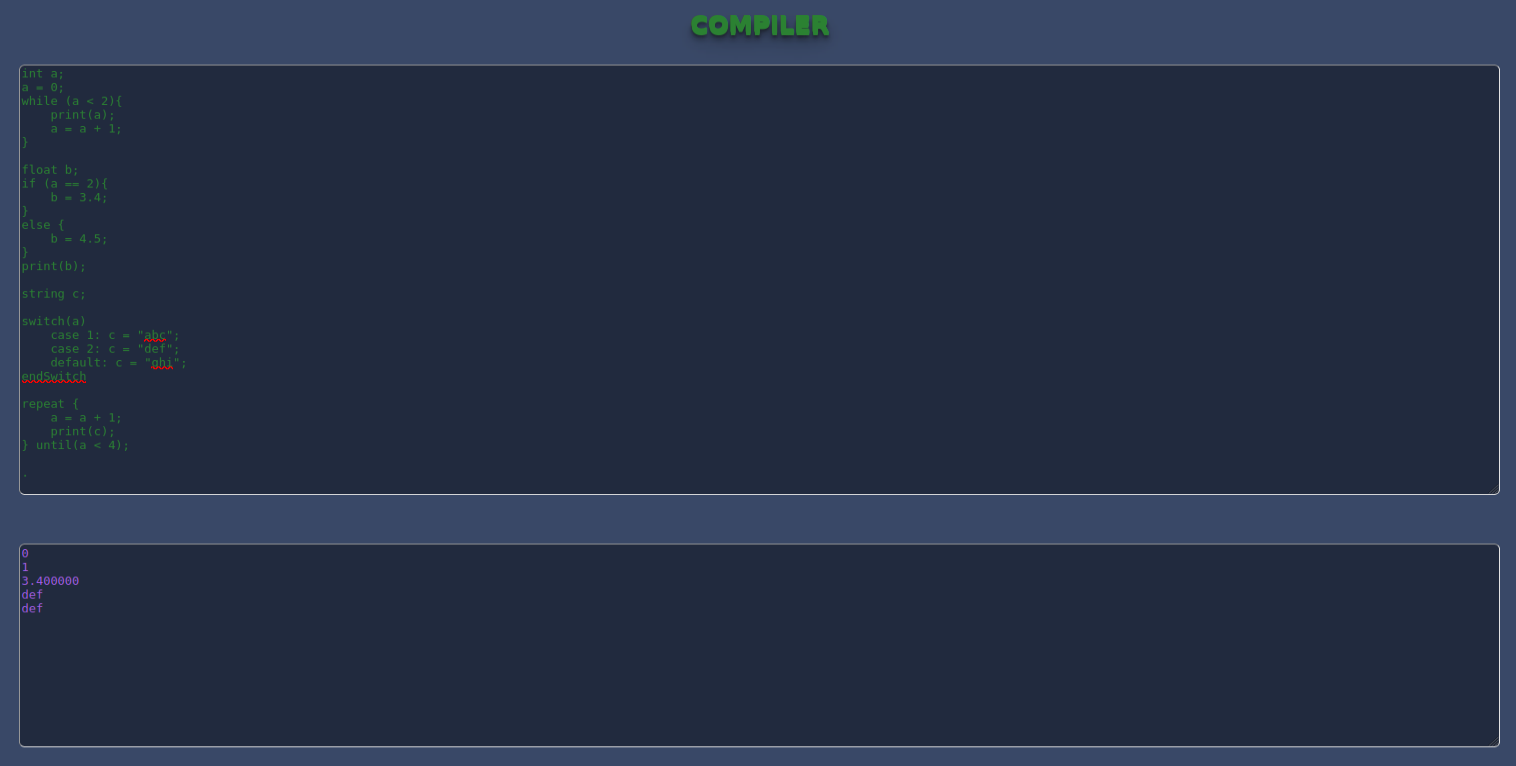
\includegraphics[scale = 0.4]{combined.png}\\
\textit{Mai multe instructiuni combinate}
\end{center}

\section{Link proiect}
\href{https://github.com/floreaneusebiu3/CODE_COMPILER}{Proiectul poate fi regasit aici.}

\end{document}
